\documentclass[tikz]{standalone}
\usepackage{pgfplots}
\pgfplotsset{compat=1.15}
\usepackage{mathrsfs}
\usetikzlibrary{arrows,calc}
\usepackage{tkz-euclide}
\pagestyle{empty}

\definecolor{AngleClr}{rgb}{0,0.39215686274509803,0}
\definecolor{ShapeClr}{rgb}{0.6,0.2,0}
\definecolor{BlueSqr}{RGB}{5,81,163}
\definecolor{RedSqr}{RGB}{0, 156, 0}

\begin{document}

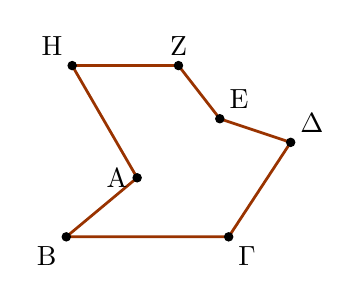
\begin{tikzpicture}[scale=.75]
\tkzSetUpLine[line width=1pt,color=black]
\tkzSetUpPoint[fill=black]

\tkzDefPoints{0/0/B,2.75/0/C,1.2/1/A,0.1/2.9/G,1.9/2.9/F,2.6/2/E,3.8/1.6/D}

\tkzFillPolygon[fill=white](A,B,C,D,E,F,G)

\tkzDrawPolygon[color=ShapeClr](A,B,C,D,E,F,G)
\tkzDrawPoints[size=3](A,B,C,D,E,F,G)
\tkzLabelPoint[left](A){$\mathrm{A}$}
\tkzLabelPoint[below left](B){$\rm B$}
\tkzLabelPoint[below right](C){$\rm \Gamma$}
\tkzLabelPoint[above right](D){$\rm \Delta$}
\tkzLabelPoint[above right](E){$\rm E$}
\tkzLabelPoint[above](F){$\rm Z$}
\tkzLabelPoint[above left](G){$\rm H$}

\end{tikzpicture}

\end{document}
